\documentclass{extreport}

\usepackage[14pt]{extsizes}
\usepackage[T2A]{fontenc}
\usepackage[utf8]{inputenc}
\usepackage[english,ukrainian]{babel}

\usepackage[a4paper, top=10mm, bottom=15mm, left=20mm, right=15mm]{geometry}
\usepackage{amsmath,amsfonts,amssymb,amsthm,mathtools}
\usepackage{listings}
\usepackage{graphicx}
\usepackage{enumitem}
\usepackage{verbatim}
\usepackage{listings}
\usepackage{xcolor}
\usepackage{textgreek}
\usepackage{diagbox}
\usepackage{pgfplots}
\pgfplotsset{compat = 1.17}


\lstdefinestyle{output_txt}{
    basicstyle=\ttfamily\footnotesize,
    breakatwhitespace=false,         
    breaklines=true,                 
    captionpos=b,                    
    keepspaces=true,                                    
    numbersep=5pt,                  
    showspaces=false,                
    showstringspaces=false,
    showtabs=false,                  
    tabsize=2
}
\definecolor{codegreen}{rgb}{0,0.6,0}
\definecolor{codegray}{rgb}{0.5,0.5,0.5}
\definecolor{codepurple}{rgb}{0.58,0,0.82}
\lstdefinestyle{python_code}{ 
    commentstyle=\color{codegreen},
    keywordstyle=\color{magenta},
    numberstyle=\tiny\color{codegray},
    stringstyle=\color{codepurple},
    basicstyle=\ttfamily\footnotesize,
    breakatwhitespace=false,         
    breaklines=true,                 
    captionpos=b,                    
    keepspaces=true,                            
    numbersep=5pt,                  
    showspaces=false,                
    showstringspaces=false,
    showtabs=false,                  
    tabsize=4
}

\setlist[enumerate]{nosep}
\graphicspath{{pics/}}
\DeclareGraphicsExtensions{.png}

\begin{document}
\begin{titlepage}
    \thispagestyle{empty}
    \begin{center}
        
\includegraphics[width = \textwidth]{kpi}
        Міністерство освіти і науки України\\
        Національний технічний університет України\\
        <<Київський політехнічний інститут ім. І. Сікорського>>\\
        Інститут прикладного системного аналізу
    \end{center}
    \vspace{40mm}
    \begin{center}
        \textbf{Лабораторна робота} \\
        з курсу <<Методи оптимізації>> \\
        з теми <<Чисельні методи безумовної оптимізації першого порядку. 
        Градієнтний метод та його варіації>>
    \end{center}
    \vspace{20mm}
    \begin{flushleft}
        Виконали студенти 3 курсу групи КА-81 \\
        Галганов Олексій \\
        Єрко Андрій \\
        Фордуй Нікіта
    \end{flushleft}
    \begin{flushright}
        Перевірили \\
        Спекторський Ігор Якович \\
        Яковлева Алла Петрівна
    \end{flushright}
    \vspace{30mm}
    \begin{center}
        \textbf{Київ 2021}
    \end{center}
\end{titlepage}

\begin{center}
    \textbf{Варіант 1}
\end{center}
\textbf{Завдання.} Скласти програму для мінімізації цільової функції
одним з градієнтних методів. Конкретний тип градієнтного методу обрати
самостійно, ураховуючи особливості цільової функції.

\emph{Цільова функція:}
$f(x,y) = x^2 + 18y^2 + 0.01xy + x - y$

\noindent\textbf{Результати роботи.}
Для визначення ярності цільової функції розглянемо її матрицю Гессе
$f''(x,y) = \begin{pmatrix}
    2 & 0.01 \\
    0.01 & 36
\end{pmatrix}$. Її власні числа приблизно рівні 2 та 36, тому матриця є погано обумовленою.
Також це видно з графіку цільової функції та її ліній рівня.
\begin{center}
    \begin{tabular}{c c}
        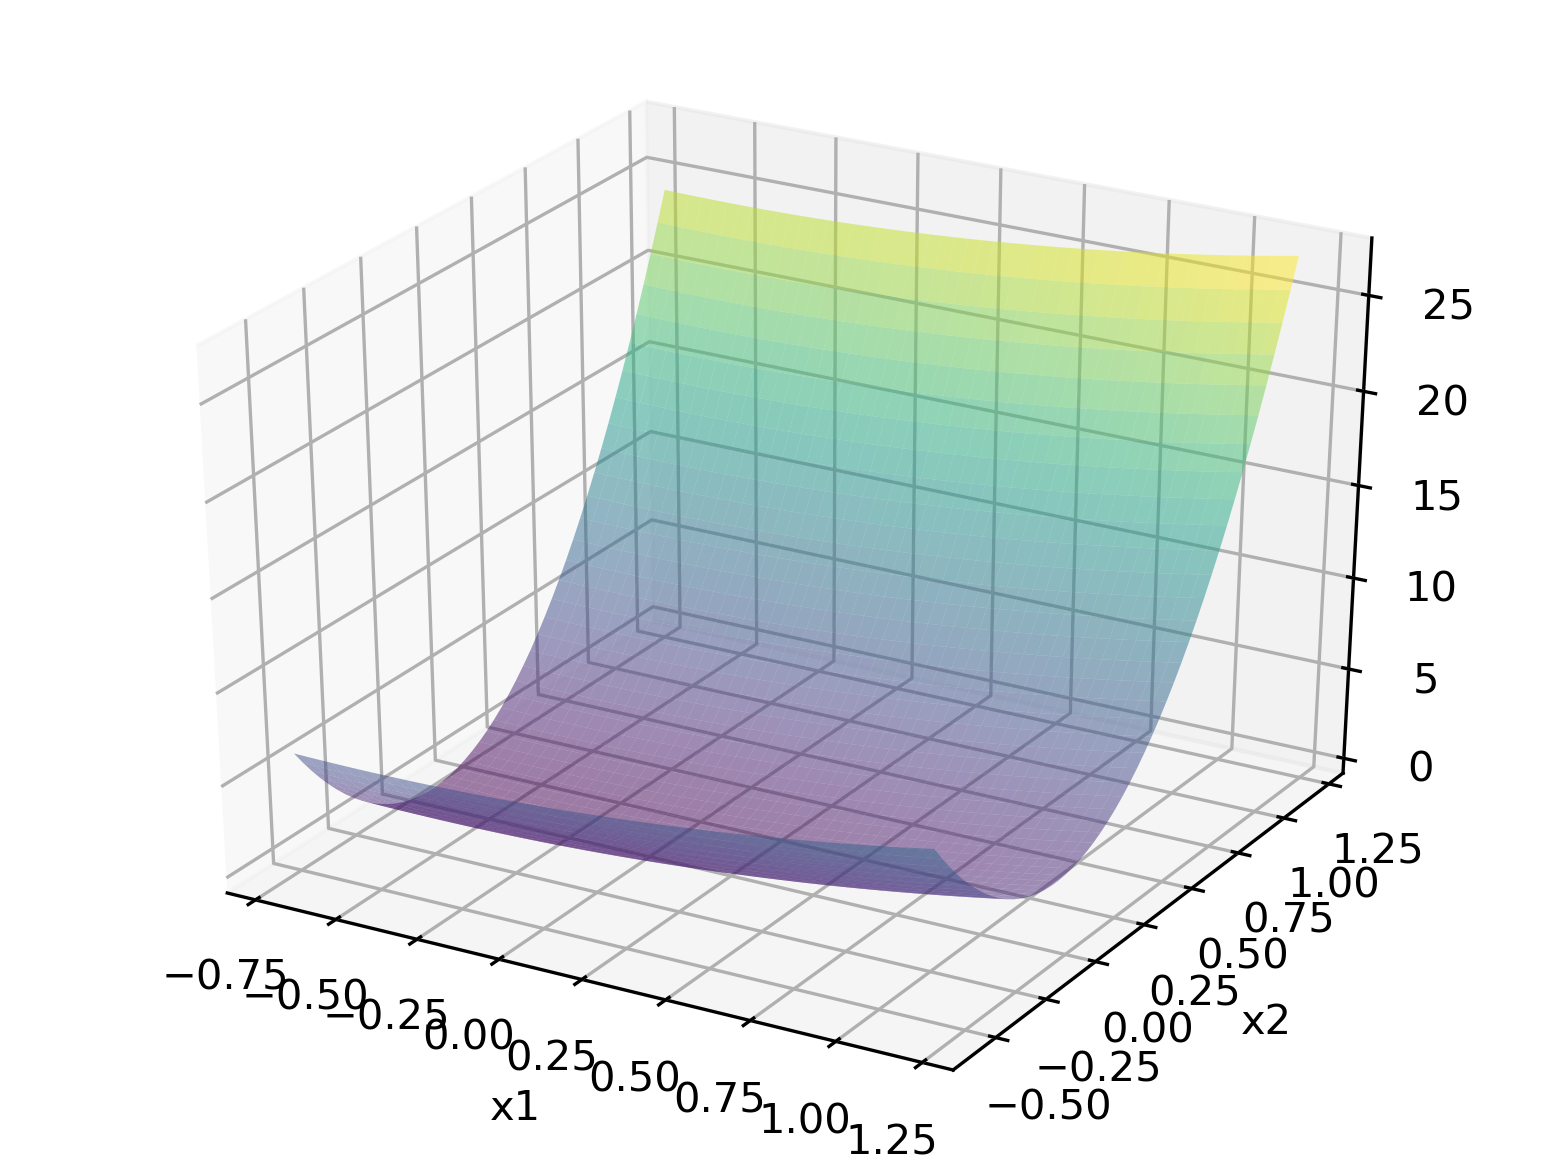
\includegraphics[scale = 0.6]{surface_init.png} &
        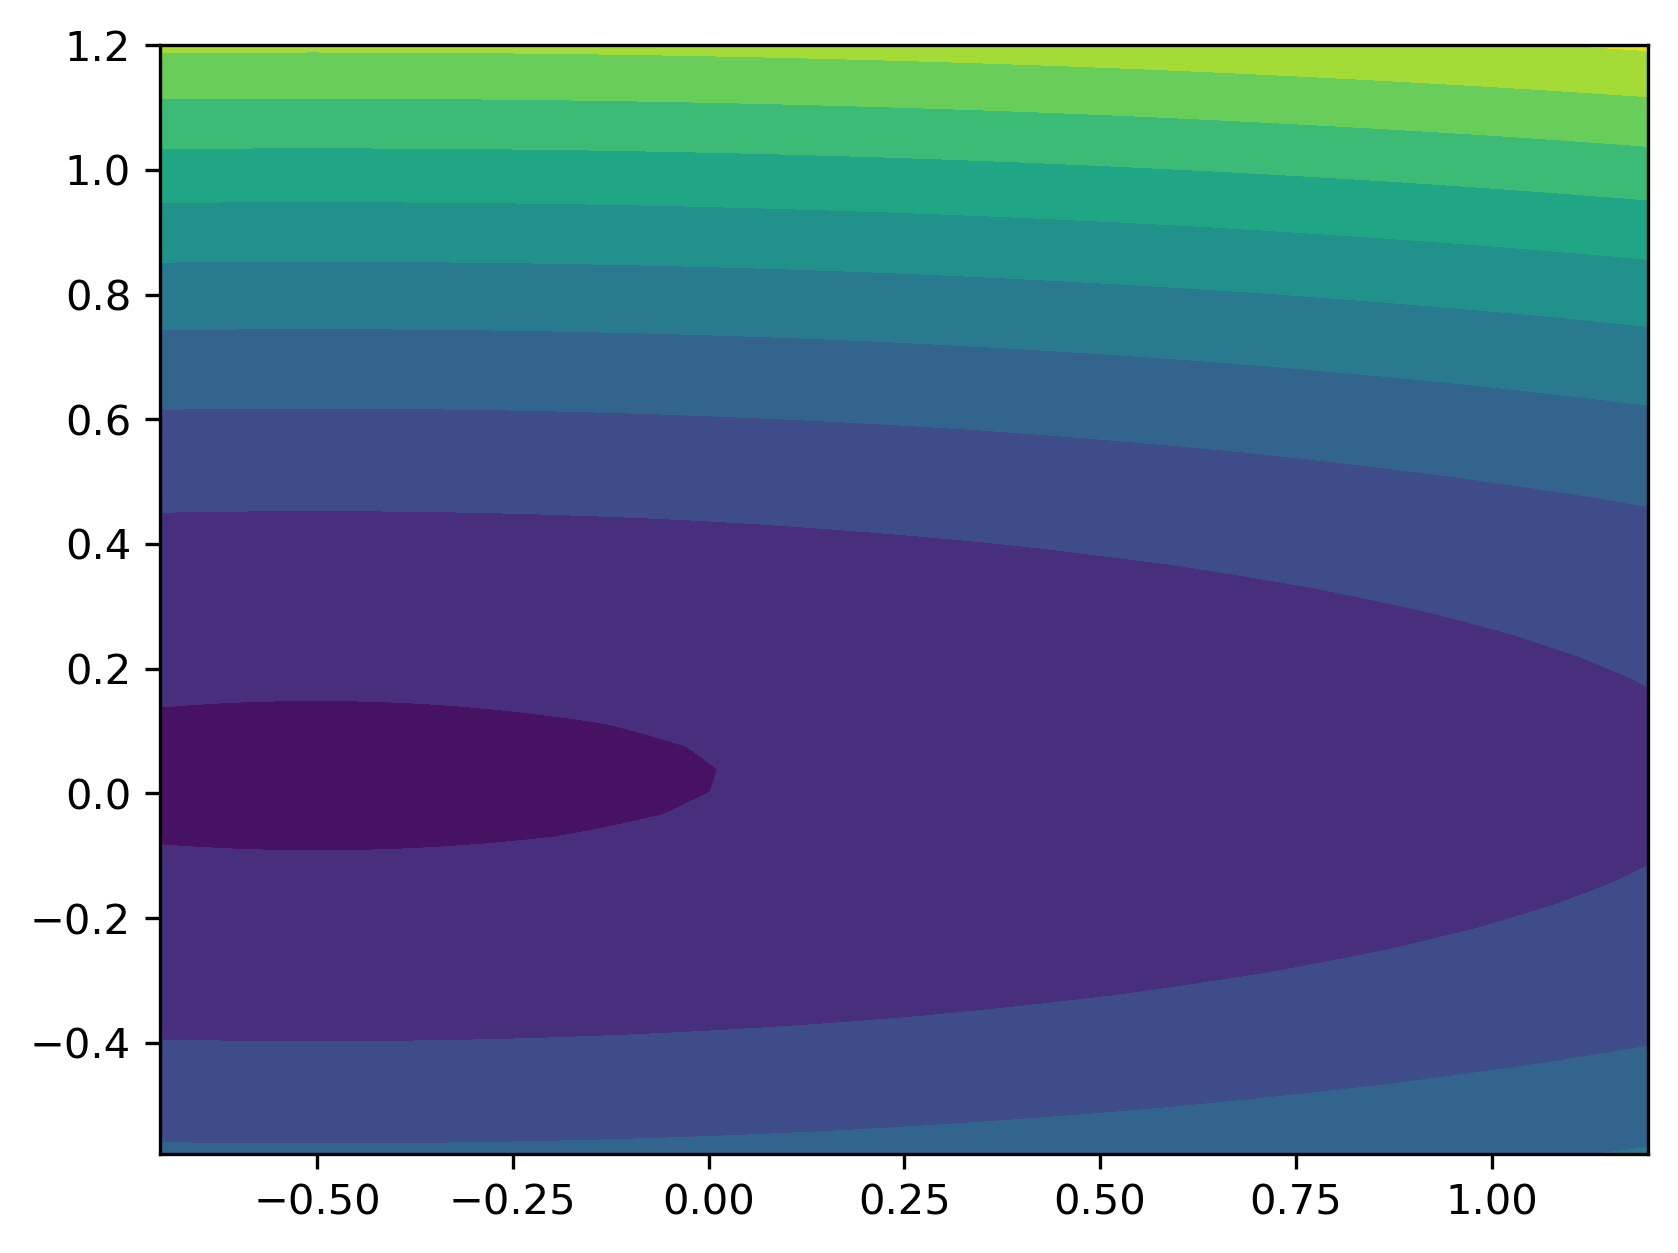
\includegraphics[scale = 0.5]{contour_init.png}
    \end{tabular}
\end{center}
Отже, функція має <<ярну>> структуру, тому для прискорення
збіжності необхідно застосувати якусь модифікацію градієнтного методу.
Для реалізації було обрано метод дроблення кроку, який має допомогти зменшити 
зигзагоподібний характер шляху до точки мінімуму.
Обраний критерій зупинки --- $\left| f(x_{k+1}) - f(x_k)\right| < \varepsilon = 10^{-5}$.
Було отримано збіжність до точки мінімуму за 55 ітерацій.
\begin{center}
    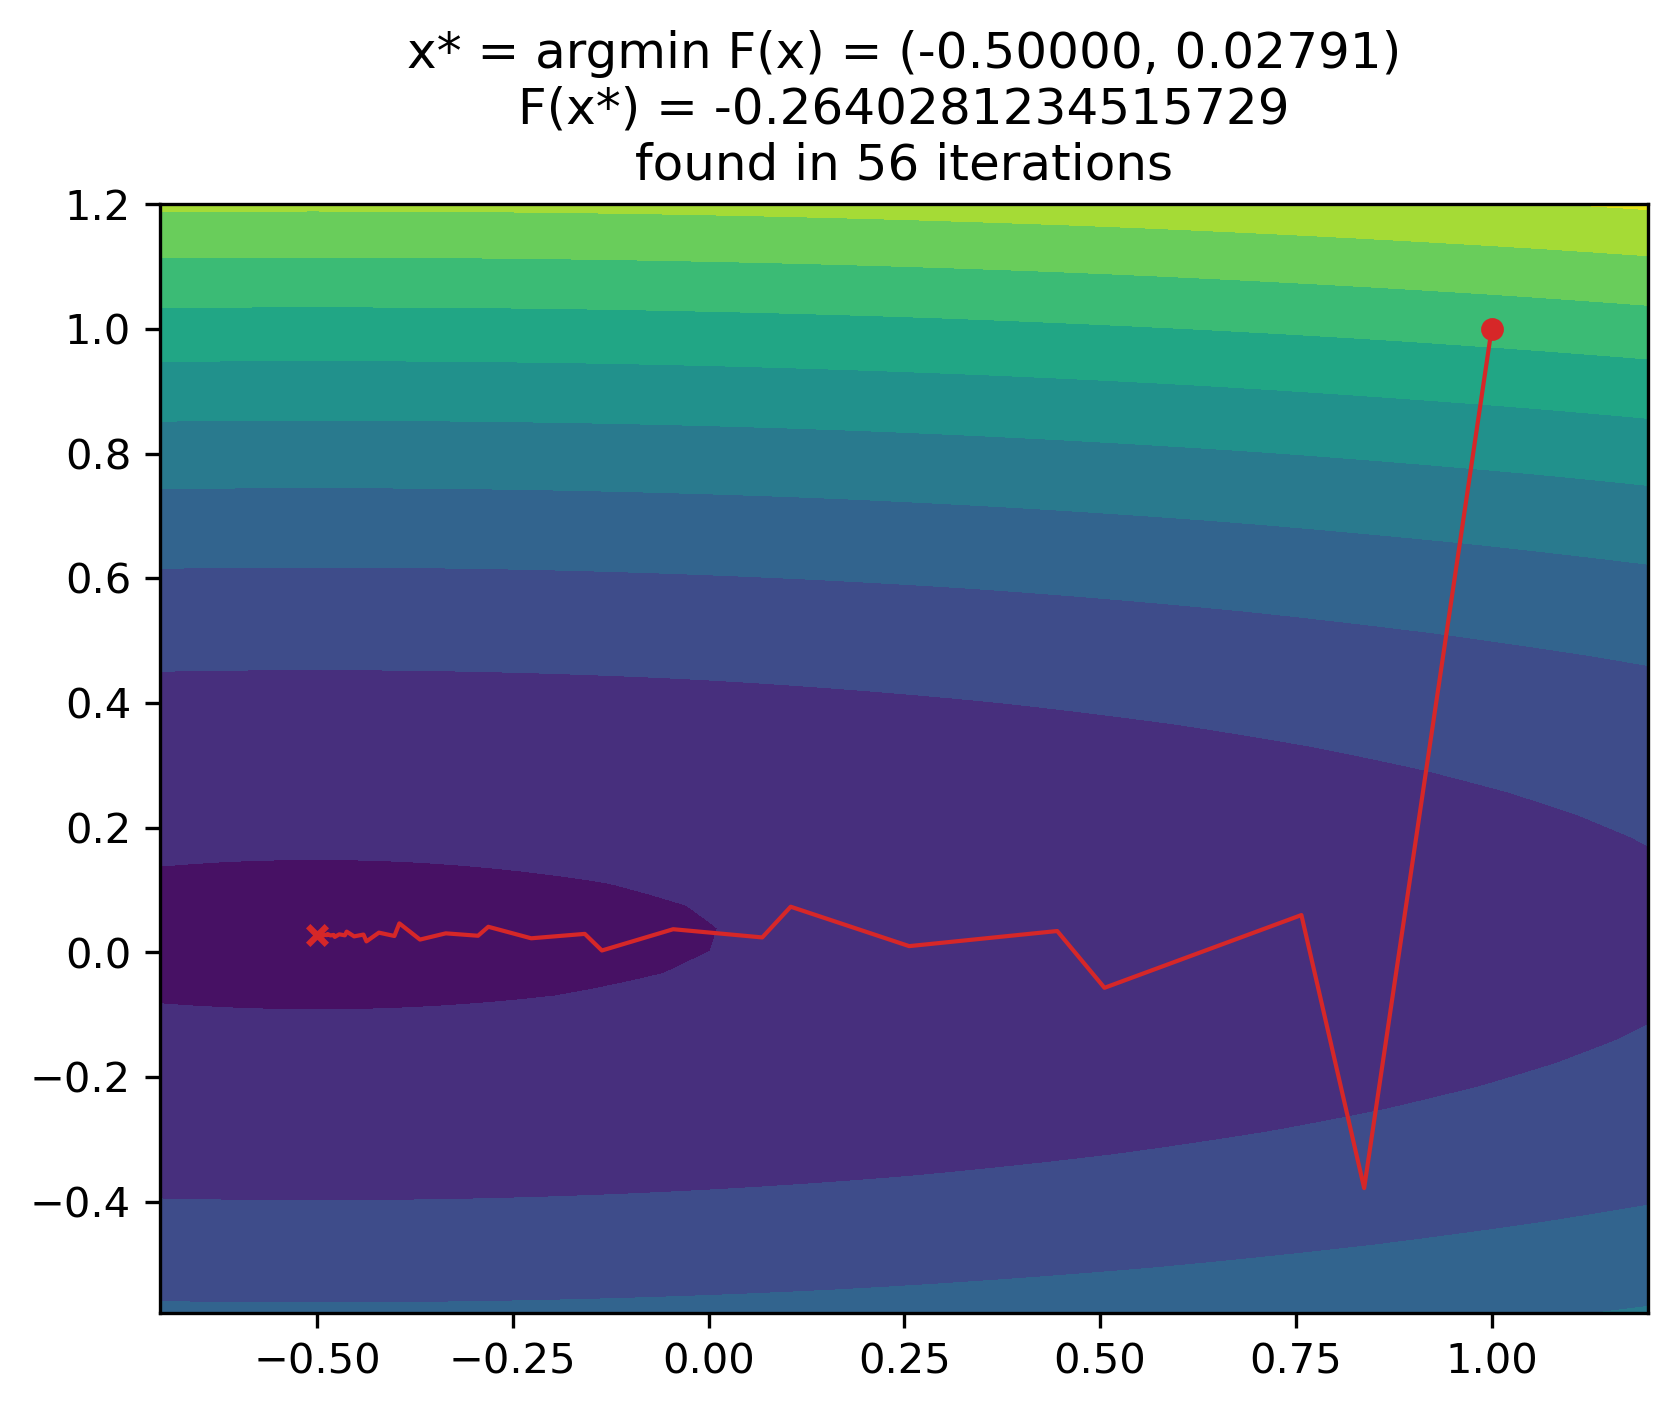
\includegraphics[scale = 0.8]{contour_final.png}
\end{center}

\noindent\textbf{Лістинг.}
Текст програми було розділено на \texttt{Optimizer.py} з реалізацією
власне градієнтного методу та \texttt{lab1.py}, де він викликається та зберігаються результати.

\noindent\texttt{Optimizer.py}
\lstinputlisting[language = Python, style = python_code]{../code/Optimizer.py}

\noindent\texttt{lab1.py}
\lstinputlisting[language = Python, style = python_code]{../code/lab1.py}

\noindent\textbf{Висновки.} При виконанні даної роботи ми дослідили
застосування градієнтного методу до мінімізації заданої квадратичної функції, що має
ярну структуру. Для збільшення швидкості збіжності було реалізовано метод дроблення кроку,
який на кожній ітерації обирає крок $\alpha_k$ найбільшим серед тих, які забезпечують рух
у напрямку мінімуму.
\end{document}